\label{attachment:comparisons}

\begin{figure}[htbp]
    \centering
    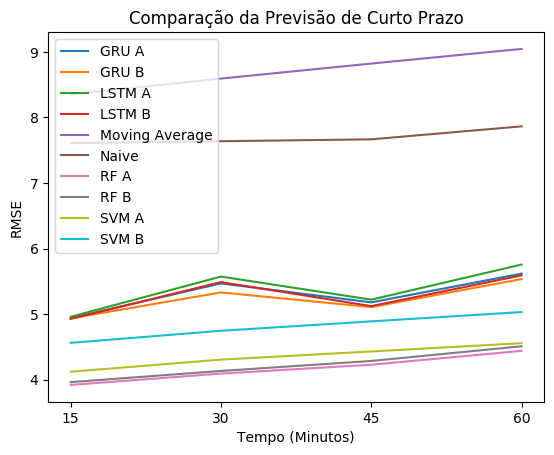
\includegraphics[scale=0.8]{monography/img/comparisons/comparacao_da_previsao_de_curto_prazo_rmse.png}
    \label{figure:previsao_de_curto_prazo_rmse}
    \caption{Comparação de previsão de curto prazo sem ajuste de hiper-parâmetros utilizando RMSE}
\end{figure}

\begin{figure}[htbp]
    \centering
    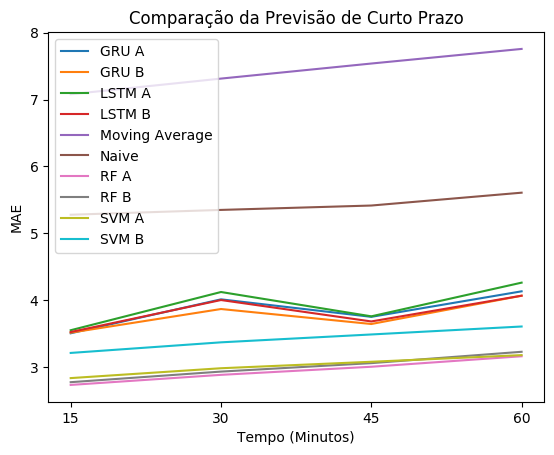
\includegraphics[scale=0.8]{monography/img/comparisons/comparacao_da_previsao_de_curto_prazo_mae.png}
    \label{figure:previsao_de_curto_prazo_mae}
    \caption{Comparação de previsão de curto prazo sem ajuste de hiper-parâmetros utilizando MAE}
\end{figure}

\begin{figure}[htbp]
    \centering
    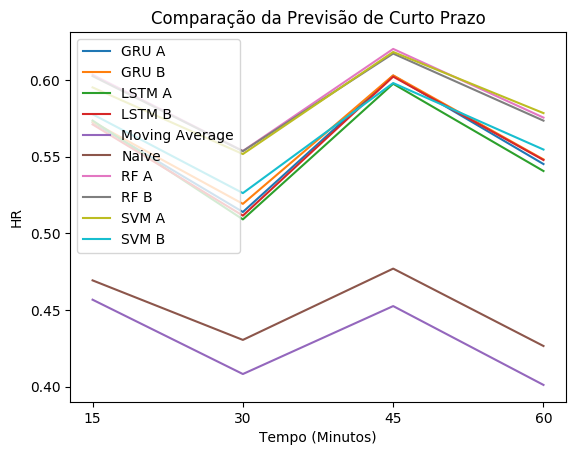
\includegraphics[scale=0.8]{monography/img/comparisons/comparacao_da_previsao_de_curto_prazo_hr.png}
    \label{figure:previsao_de_curto_prazo_hr}
    \caption{Comparação de previsão de curto prazo sem ajuste de hiper-parâmetros utilizando precisão}
\end{figure}

\begin{figure}[htbp]
    \centering
    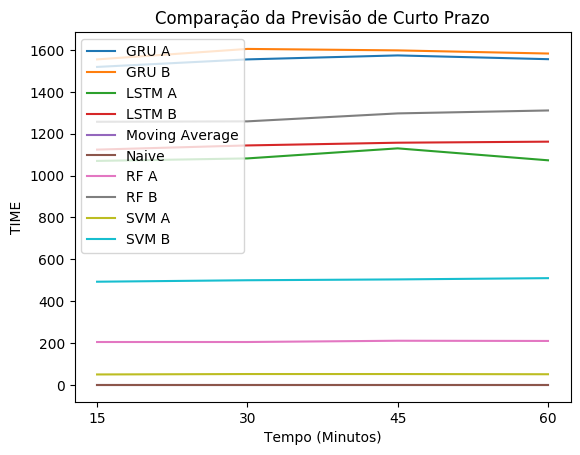
\includegraphics[scale=0.8]{monography/img/comparisons/comparacao_da_previsao_de_curto_prazo_time.png}
    \label{figure:previsao_de_curto_prazo_time}
    \caption{Comparação de previsão de curto prazo sem ajuste de hiper-parâmetros utilizando tempo de treinamento}
\end{figure}

\begin{figure}[htbp]
    \centering
    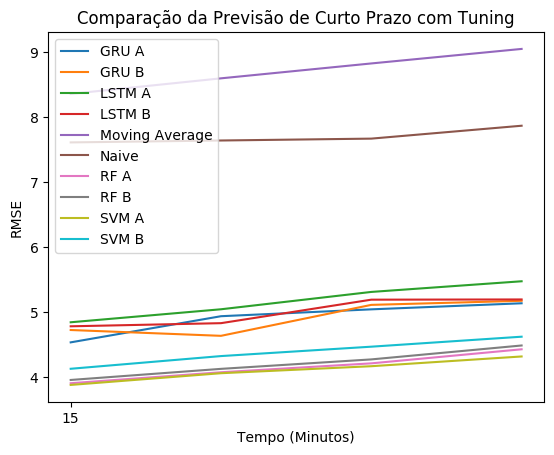
\includegraphics[scale=0.8]{monography/img/comparisons/comparacao_da_previsao_de_curto_prazo_com_tuning_rmse.png}
    \label{figure:previsao_de_curto_prazo_com_tuning_rmse}
    \caption{Comparação de previsão de curto prazo com ajuste de hiper-parâmetros utilizando RMSE}
\end{figure}

\begin{figure}[htbp]
    \centering
    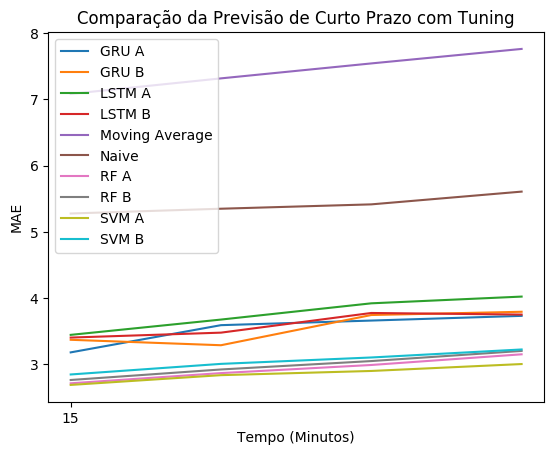
\includegraphics[scale=0.8]{monography/img/comparisons/comparacao_da_previsao_de_curto_prazo_com_tuning_mae.png}
    \label{figure:previsao_de_curto_prazo_com_tuning_mae}
    \caption{Comparação de previsão de curto prazo com ajuste de hiper-parâmetros utilizando MAE}
\end{figure}

\begin{figure}[htbp]
    \centering
    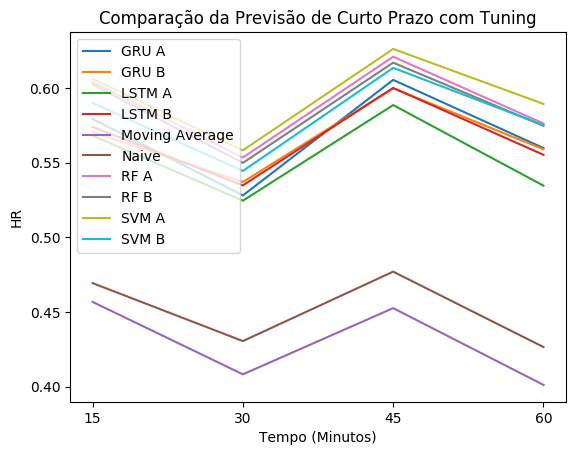
\includegraphics[scale=0.8]{monography/img/comparisons/comparacao_da_previsao_de_curto_prazo_com_tuning_hr.png}
    \label{figure:previsao_de_curto_prazo_com_tuning_hr}
    \caption{Comparação de previsão de curto prazo com ajuste de hiper-parâmetros utilizando precisão}
\end{figure}

\begin{figure}[htbp]
    \centering
    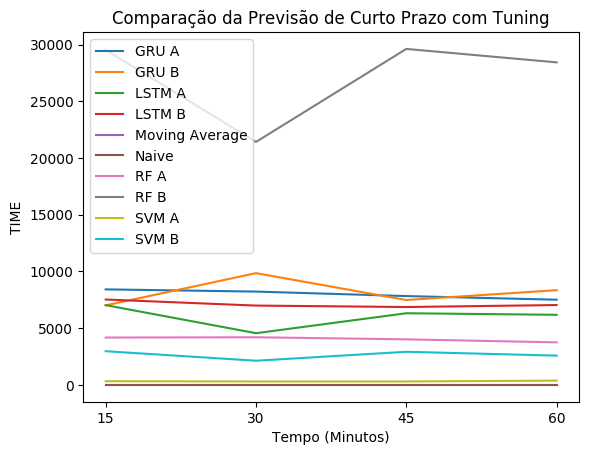
\includegraphics[scale=0.8]{monography/img/comparisons/comparacao_da_previsao_de_curto_prazo_com_tuning_time.png}
    \label{figure:previsao_de_curto_prazo_com_tuning_time}
    \caption{Comparação de previsão de curto prazo com ajuste de hiper-parâmetros utilizando tempo de treinamento}
\end{figure}

% \section{Número de Divisões do Conjunto de Dados}

\begin{figure}[htbp]
    \centering
    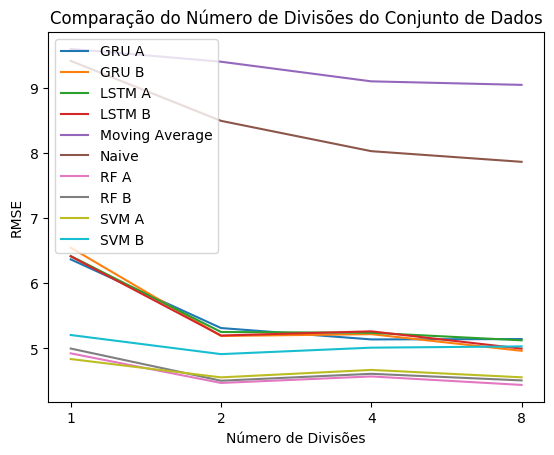
\includegraphics[scale=0.8]{monography/img/comparisons/comparacao_do_numero_de_divisoes_do_conjunto_de_dados_rmse.png}
    \label{figure:numero_de_divisoes_do_conjunto_de_dados_rmse}
    \caption{Comparação do número de divisões do conjunto de dados utilizando RMSE}
\end{figure}

\begin{figure}[htbp]
    \centering
    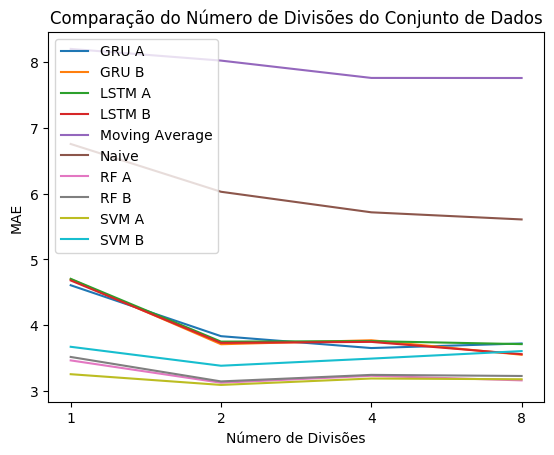
\includegraphics[scale=0.8]{monography/img/comparisons/comparacao_do_numero_de_divisoes_do_conjunto_de_dados_mae.png}
    \label{figure:numero_de_divisoes_do_conjunto_de_dados_mae}
    \caption{Comparação do número de divisões do conjunto de dados utilizando MAE}
\end{figure}

\begin{figure}[htbp]
    \centering
    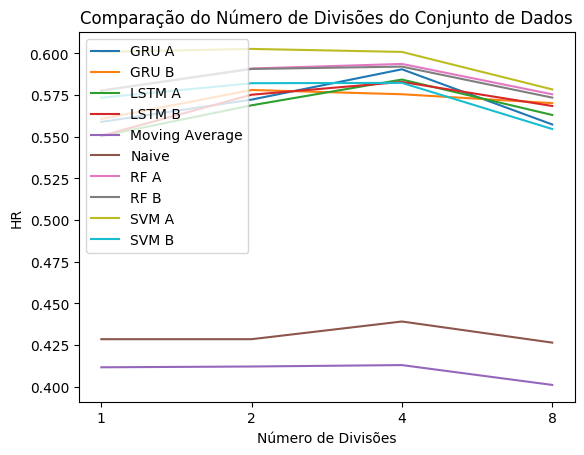
\includegraphics[scale=0.8]{monography/img/comparisons/comparacao_do_numero_de_divisoes_do_conjunto_de_dados_hr.png}
    \label{figure:numero_de_divisoes_do_conjunto_de_dados_hr}
    \caption{Comparação do número de divisões do conjunto de dados utilizando precisão}
\end{figure}

\begin{figure}[htbp]
    \centering
    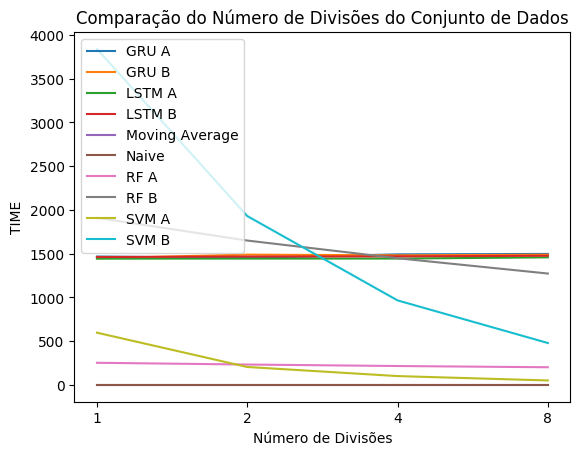
\includegraphics[scale=0.8]{monography/img/comparisons/comparacao_do_numero_de_divisoes_do_conjunto_de_dados_time.png}
    \label{figure:numero_de_divisoes_do_conjunto_de_dados_time}
    \caption{Comparação do número de divisões do conjunto de dados utilizando tempo de treinamento}
\end{figure}

\begin{figure}[htbp]
    \centering
    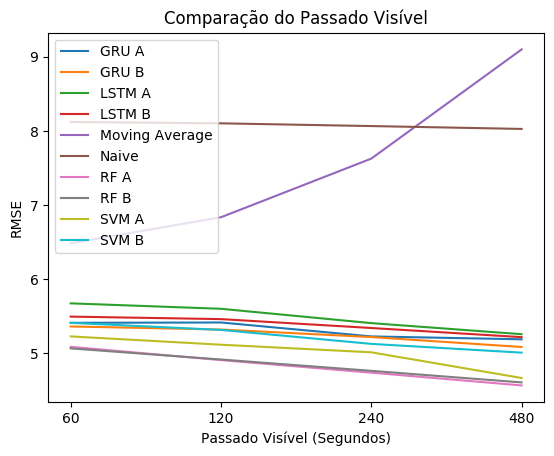
\includegraphics[scale=0.8]{monography/img/comparisons/comparacao_do_passado_visivel_rmse.png}
    \label{figure:passado_visivel_rmse}
    \caption{Comparação do passado visível utilizando RMSE}
\end{figure}

\begin{figure}[htbp]
    \centering
    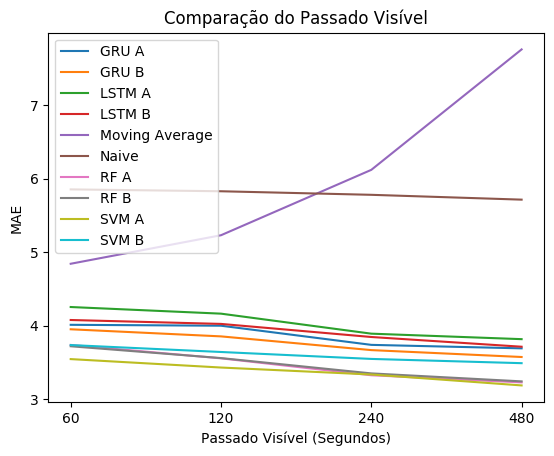
\includegraphics[scale=0.8]{monography/img/comparisons/comparacao_do_passado_visivel_mae.png}
    \label{figure:passado_visivel_mae}
    \caption{Comparação do passado visível utilizando MAE}
\end{figure}

\begin{figure}[htbp]
    \centering
    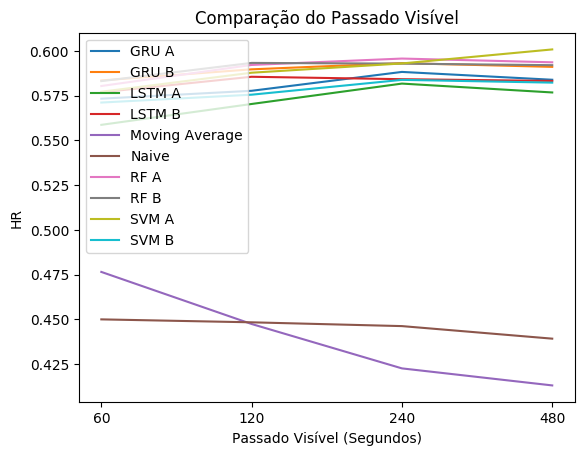
\includegraphics[scale=0.8]{monography/img/comparisons/comparacao_do_passado_visivel_hr.png}
    \label{figure:passado_visivel_hr}
    \caption{Comparação do passado visível utilizando precisão}
\end{figure}

\begin{figure}[htbp]
    \centering
    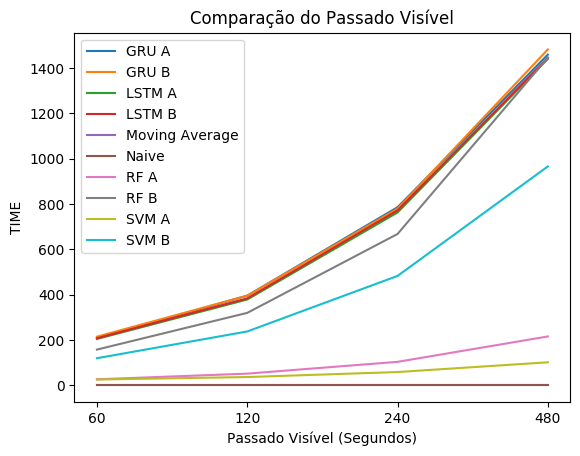
\includegraphics[scale=0.8]{monography/img/comparisons/comparacao_do_passado_visivel_time.png}
    \label{figure:passado_visivel_time}
    \caption{Comparação do passado visível utilizando tempo de treinamento}
\end{figure}

% \section{Tamanho do Intervalo do Fluxo}

\begin{figure}[htbp]
    \centering
    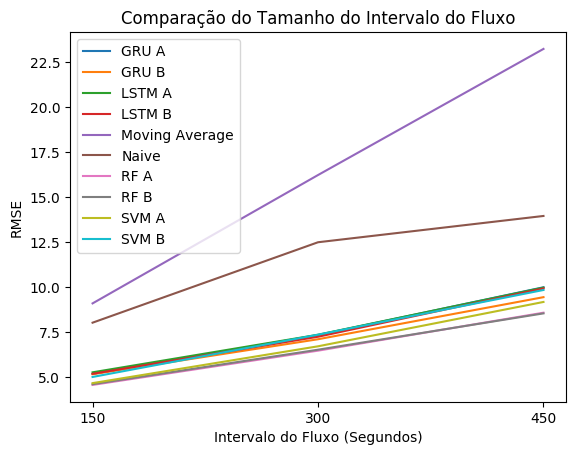
\includegraphics[scale=0.8]{monography/img/comparisons/comparacao_do_tamanho_do_intervalo_do_fluxo_rmse.png}
    \label{figure:tamanho_do_intervalo_do_fluxo_rmse}
    \caption{Comparação do tamanho do intervalo do fluxo utilizando RMSE}
\end{figure}

\begin{figure}[htbp]
    \centering
    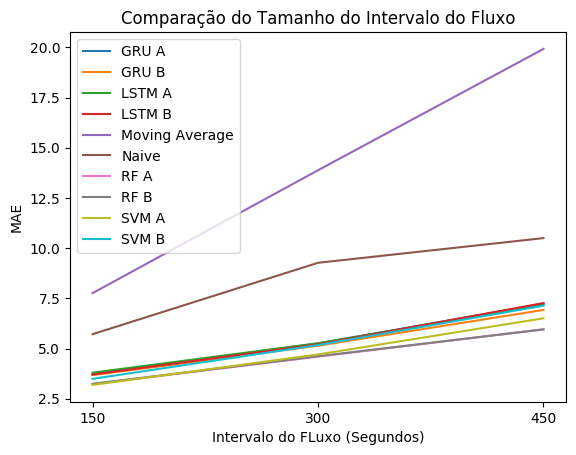
\includegraphics[scale=0.8]{monography/img/comparisons/comparacao_do_tamanho_do_intervalo_do_fluxo_mae.png}
    \label{figure:tamanho_do_intervalo_do_fluxo_mae}
    \caption{Comparação do tamanho do intervalo do fluxo utilizando MAE}
\end{figure}

\begin{figure}[htbp]
    \centering
    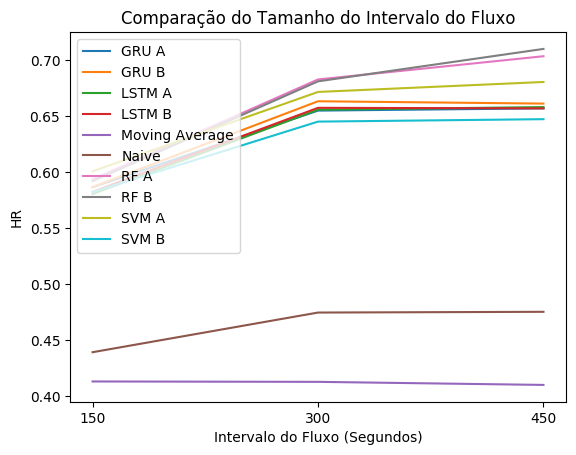
\includegraphics[scale=0.8]{monography/img/comparisons/comparacao_do_tamanho_do_intervalo_do_fluxo_hr.png}
    \label{figure:tamanho_do_intervalo_do_fluxo_hr}
    \caption{Comparação do tamanho do intervalo do fluxo utilizando precisão}
\end{figure}

\begin{figure}[htbp]
    \centering
    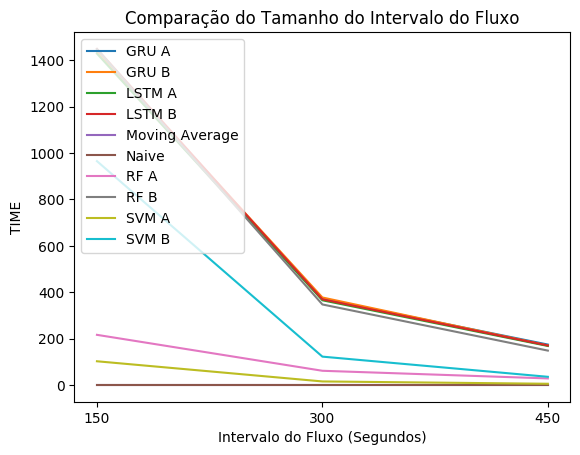
\includegraphics[scale=0.8]{monography/img/comparisons/comparacao_do_tamanho_do_intervalo_do_fluxo_time.png}
    \label{figure:tamanho_do_intervalo_do_fluxo_time}
    \caption{Comparação do tamanho do intervalo do fluxo utilizando tempo de treinamento}
\end{figure}